\chapter{An Overview of KLARAPTOR}
\label{ch:overview}

In this chapter, we present an overview of KLARAPTOR, a compile-time tool designed to optimize the performance of 
CUDA kernels by dynamically choosing the most suitable thread block configuration. We discuss the underlying theory 
of rational programs and the MWP-CWP performance model, which form the basis of KLARAPTOR's functionality. Furthermore, 
we explain the process of building and utilizing rational programs to determine optimal kernel launch parameters, 
detailing both the compile-time and runtime aspects of the tool. This chapter aims to provide an in-depth understanding of 
KLARAPTOR's methodology and how it contributes to enhancing kernel performance in CUDA applications.

\section{Dynamic Optimization of CUDA Kernel Launch Parameters}
\label{sec:klaraptor}

%\begin{figure*}[ht]
%	\centering
%	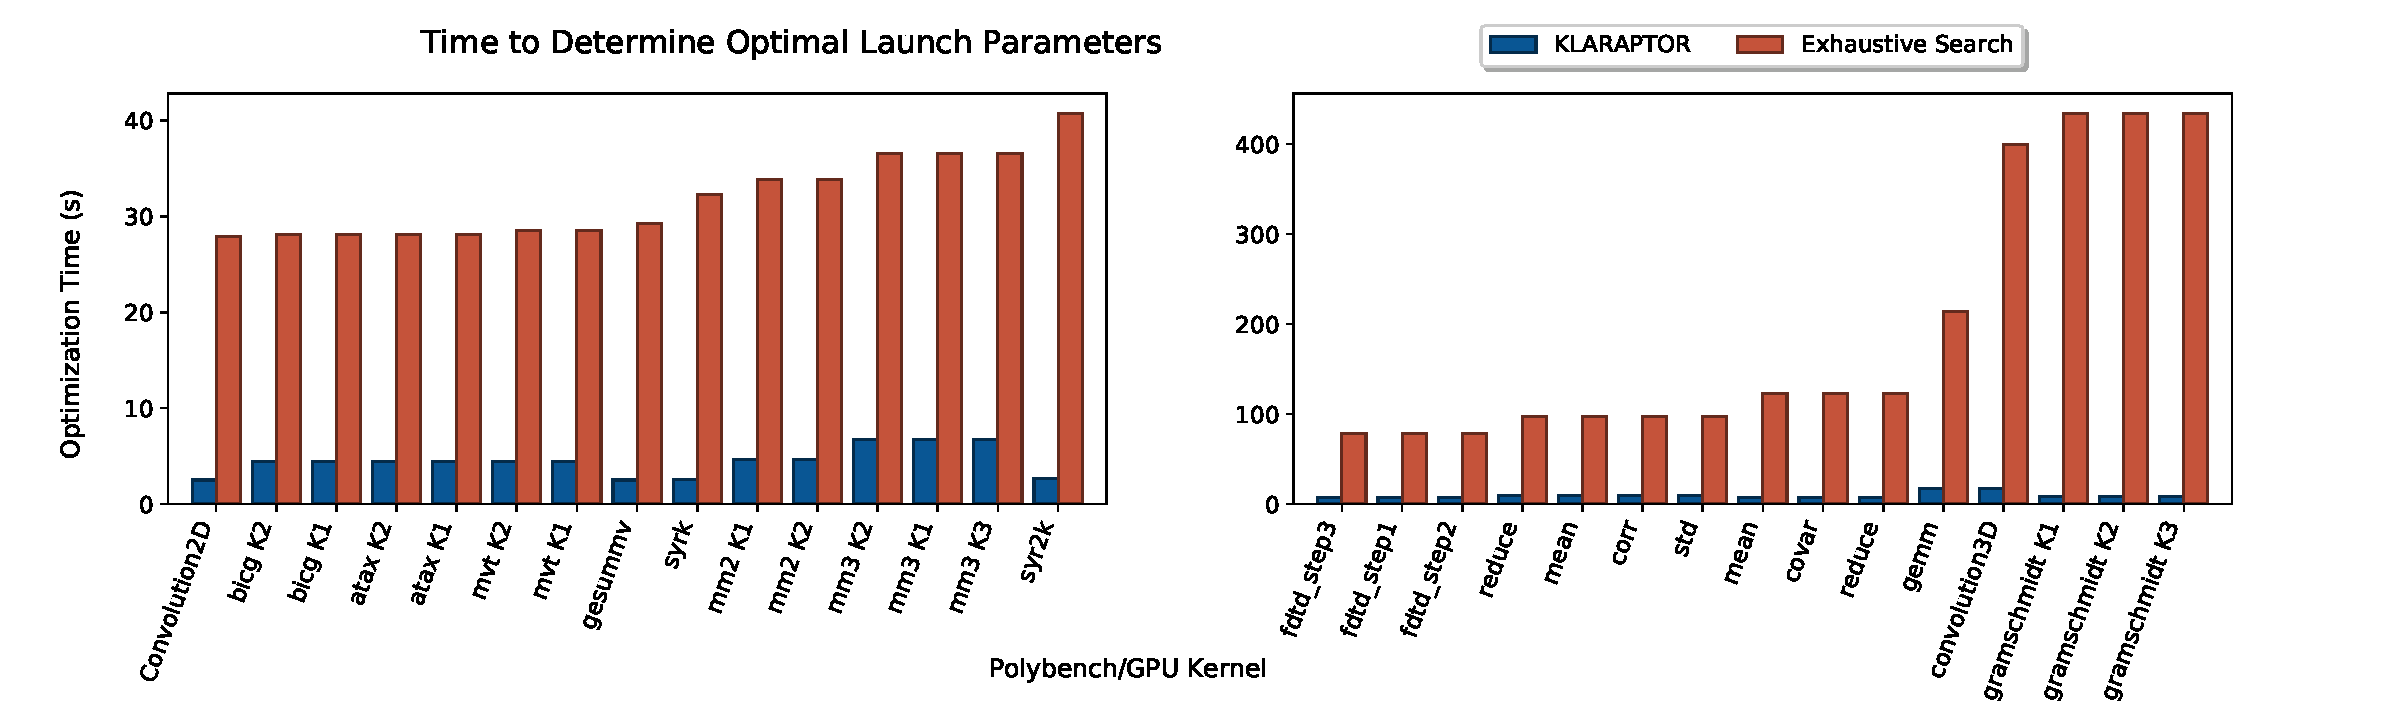
\includegraphics[width=\textwidth,clip,trim={1.5em, 1em, 5.5em, 1.2em}]{Figures/SystemTimesAll.pdf}
%	\caption{Comparing cumulative times to determine optimal launch parameters for data sizes $32 \leq N \leq 2048$ for each kernel in \texttt{Polybench/GPU}.}\label{fig:systemtimesall}
%\end{figure*}

The theory of rational programs is put into practice for the {\cuda}
programming model by our tool KLARAPTOR.  KLARAPTOR is a compile-time
tool implemented using the LLVM Pass Framework and the {\mwpcwp}
performance model to dynamically choose a {\cuda} kernel's launch
parameters (thread block configuration) which optimize its
performance.  Most high-performance computing applications require
computations be as fast as possible and so kernel performance is
simply measured as its execution time.

As mentioned in Chapter~\ref{ch:intro}, 
thread block configurations drastically affect the running time of a kernel.
Determining optimal thread block configurations typically follows some heuristics, for example, 
constraining block size to be a multiple of 32 \cite{cuda2016best}. However, it is known
that the dimension sizes of a thread block, not only its total size, affect performance~\cite{DBLP:journals/tjs/TorresGL13,DBLP:conf/cascon/ChenCKMX15}.
Moreover, since thread block configurations are intimately tied to the size of data being operated on,
it is very unlikely that a static thread block configuration optimizes the performance 
of all data sizes. Our tool effectively uses rational programs to 
dynamically determine the thread block configuration 
which minimizes the execution time of a particular 
kernel invocation, considering
the invocation's particular data size 
and target architecture. 
This is achieved in two main steps. 
\begin{enumerate}
	\item At the compile-time of a {\cuda} program, its kernels are analyzed in order to
	build rational programs estimating some performance metrics for each individual kernel.
	Each rational program, written as code in the C language,
	is inserted into the code of the {\cuda} program
	so that it is called before the execution of the corresponding kernel.
	\item At runtime, immediately preceding the launch of a kernel, where data parameters have specific values, the rational program is evaluated to 
	determine the thread block configuration which optimizes the performance of the kernel. The kernel
	is then launched using this thread block configuration. 
\end{enumerate} 

Not only are we concerned with kernel performance, but also
programmer performance. By that, 
we mean the efficiency of a programmer to produce 
optimal code. When a programmer is attempting to optimize a kernel, choosing optimal launch
parameters can either be completely ignored, 
performed heuristically, determined by trial and error, or determined by an exhaustive search.
The latter two options quickly become infeasible as data sizes grow large.
Regardless, any choice of optimal thread block configuration is likely to optimize
only a single data size. 

For KLARAPTOR to be practical, not only does the choice of optimal
kernel launch parameters need to be correct, but it must also
be more efficient than trial and error or exhaustive search.
Namely, the compile-time analysis cannot add too much 
overhead to the the compilation time and the
runtime decision of the kernel launch parameters cannot
overwhelm the program execution time. 
For the former, our analysis is performed
quickly by analyzing kernel performance on only small data sizes, 
and then results are extrapolated.
For the later, the rational program evaluation is quick and simple, 
being only the evaluation of a few rational functions.
Moreover, we maintain a runtime invocation history
to instantly provide results for future kernel launches.
Our implementation is detailed in Chapter~\ref{ch:implementation}.
%In the remainder of this section we highlight the performance of
%KLARAPTOR.

We have made use of the \texttt{Polybench/GPU}
benchmark suite as an empirical
evaluation of the correctness of our tool on a range of {\cuda} programs.
In Figure~\ref{fig:kernelperfintro} we have already seen that KLARAPTOR
accurately predicts the optimal or near-optimal thread block
configuration. 
Before presenting more detailed results and 
experimentation in Chapter~\ref{ch:performance},
we describe the steps followed by our tool
to build and use rational programs for 
determining a thread block configuration which optimizes
performance.

%Let us begin with kernel performance. 
%Other optimization techniques (see Section~\ref{sec:relatedworks})
%focus on improving the performance of a kernel by code optimizations. Our techniques
%rather focuses on simply modifying program parameters for performance. 
%focus on auto-tuning, static source code analysis, or machine learning applied to over-simplified 
%models.


\section{An Algorithm to Select Program Parameters}
\label{sec:steps}

In this section the notations and hypotheses are the same as in
Chapter~\ref{ch:foundations}.
Namely, ${\cal E}$ is a high-level performance metric for the 
multithreaded program ${\cal P}$, 
${\bm L}$ is a set of low-level metrics of size $\ell$,
and ${\bm P}$, ${\bm D}$, ${\bm H}$ are
sets of program, data, and hardware parameters, respectively. 
Recall ${\bm P}$ has size $p$.
%%
Let us assume that the values of ${\bm H}$ are known at the compile-time of ${\cal P}$
while the values of ${\bm D}$ are known at runtime.
Further, let us assume that ${\bm P}$ and ${\bm D}$
take integer values. 
Hence the values of ${\bm P}$ belong to a finite set $F \subset \mathbb{Z}^p$.
%
%
%In particular, we assume that:
%\begin{enumerateshort}
%\item[$(i)$] ${\cal E}$
%is a high-level performance metric for the multithreaded program ${\cal P}$
%(e.g. execution time, memory
%consumption, and hardware occupancy),
%\item[$(ii)$] ${\cal E}$ is given (by a program execution model, e.g. {\cuda}
%or MWP-CWP) as a rational program depending on hardware parameters
%${\bm{H}}$, low-level performance metrics $\bm{L}$, and program parameters $\bm{P}$ (see Examples~\ref{ex:cuda} 
%and \ref{ex:mwpcwp}),
%\item[$(iii)$] the values of the hardware parameters %$H_1, \ldots, H_h$
%are known at compile-time for ${\cal P}$
%while the values of the data parameters $\bm{D}$
%are known at runtime for ${\cal P}$, 
%\item[$(iv)$] the data and program parameters 
%%$\bm{D}$, $\bm{P}$
%take integer values.
%\end{enumerateshort}
%%%
%Extending $(iv)$ we further assume that the possible values of 
%the program
%parameters $\bm{P}$ belong to a finite set $F \,\subset\, \mathbb{Z}^p$.
That is to say, the possible values of
$\bm{P}$ are tuples of the form $(\pi_1, \ldots, \pi_p) \in F$,
with each $\pi_i$ being an integer.
Let us call such a tuple a \textit{configuration} of the program parameters.
Due to the nature of program parameters, those are not necessarily all
independent variables 
%(i.e. a program parameter may depend on the value of
%another program parameter). 
%For example, in {\cuda} the product of thread block dimensions should be a power of 32.
For example, in {\cuda}, the product of the dimension sizes
of a thread block is usually
%\begin{inparaenum}[(i)]
%\item 
a multiple of the warp size (32).
%, and
%\item 
%bounded by the maximum number of threads per block.
%\end{inparaenum}

Given a performance-prediction model for ${\cal E}$, 
one could work recursively to determine a 
single helper program ${\cal R}$, depending on only
$\bm{D}$ and $\bm{P}$, evaluating ${\cal E}$,
from a combination of rational programs constructed
for each low-level metric in $\bm{L}$
and values of $\bm{D}$ and $\bm{P}$.
Following Section~\ref{sec:prf_rp}, 
each of these helper programs are constructed by 
computing rational functions. Without loss of generality,
let us assume each low-level metric is given
by a single formula and thus a single rational function. 
Hence, we look to determine $g_1(\bm{D}, \bm{P})$,
$\ldots$, $g_{\ell}(\bm{D}, \bm{P})$ for the $\ell$ 
low-level metrics.
Finally, at runtime, given particular values of $\bm{D}$,
the helper program for ${\cal E}$ can be evaluated
for various values of $\bm{P}$ to determine
the optimal configuration.
%
%However, in the context of {\cuda} we have not
%found a particularly suitable model.
%Instead, using rational functions
%for the evaluation of some low-level performance
%metrics (e.g. amount of shared memory used per thread block),
%we follow a decision tree coupled with some heuristics
%to determine the optimal configuration.
%This specialization of our general technique to {\cuda} 
%is discussed in Section~\ref{sec:heuristics}.
%
In the remainder of this section we 
describe the general process to build
and use helper programs to determine 
optimal configurations.
%%
The entire process is decomposed into five steps:
the first three occur at compile-time and the next three 
at runtime.
%Figure~\ref{fig:sixsteps} summarizes the six steps.

\begin{enumerate}
\item \textbf{Data collection}: 
%%
To perform a curve fitting of the rational functions 
$g_1(\bm{D}, \bm{P})$, $\ldots$, $g_{\ell}(\bm{D}, \bm{P})$
we require data points to fit. These are collected by 
\begin{inparaenum}[(i)]
\item selecting a subset of $K$ points
from the space of possible values of $(\bm{D}$, $\bm{P})$; and
%%
\item executing the program ${\cal P}$, recording the values of
       the low-level performance metrics $\bm{L}$ as
       ${\bm V} = (V_1, \ldots, V_{\ell})$, at each point in $K$.
\end{inparaenum}
\fixed{The data used for executing the programs is generated randomly,
but could follow some scheme provided by the user.}{Is this correct?
Davood: Totally correct.}
%%
%%
\item \textbf{Rational function approximation}: 
%%
For each low-level metric $L_i$ we use the set of points $K$ 
and the corresponding value $V_i$ measured at each point
in order to approximate
the rational function $g_i(\bm{D},\bm{P})$.
\iflongversion
We observe that if these values
were known exactly the rational function
$g_i(\bm{D}, \bm{P})$ could be determined exactly.
In practice, however, these
\else
In practice, these
\fi
empirical values are likely to be noisy from profiling,
and/or numerical approximations.
%Hence, techniques from numerical analysis, like the method of least squares,
%must be used instead. 
Consequently, we actually determine a rational function
$\hat{g}_i(\bm{D}, \bm{P})$ which approximates
$g_i(\bm{D}, \bm{P})$.
%when evaluated at the points $K_1, \ldots, K_k$.
%%
%%
\item \textbf{Code generation}: 
%%
In order to generate the helper program ${\cal R}$, we 
proceed as follows:
\begin{enumerateshort}
\item[(i)] we convert the helper program representing 
${\cal E}$ into code, 
%say in the C programming language, 
%essentially encoding the flowchart for computing $\cal{E}$;
%%
\item[(ii)] we convert each
$\hat{g}_i(\bm{D}, \bm{P})$
into a sub-routine estimating $L_i$, and
%%
\item[(iii)] we include those sub-routines
into the code computing ${\cal E}$, which yields
the desired helper program ${\cal R}$ depending only on $\bm{D}$ and $\bm{P}$.
%%
\end{enumerateshort}
%At this point the rational program ${\cal R}$ is fully determined.
%%
%%
\item \textbf{Helper program evaluation}: 
%%
At the runtime of ${\cal P}$, the data parameters $\bm{D}$ are given
particular values.
% say ${\delta}_1, \ldots, {\delta}_d$.
For those specified values of $\bm{D}$ and for
all practically meaningful values of $\bm{P}$ from
the set $F$,\footnote{The values for
$\bm{P}$ are likely to be constrained by
the values $\bm{D}$.  For example,
if $P_1, P_2$ are the two dimension sizes of a two-dimensional
thread block of a {\cuda} kernel operating on a
square matrix of order $D_1$, then $P_1 P_2 \leq D_1^2$
is meaningful.} we compute an estimate of ${\cal E}$ using ${\cal R}$.
The evaluation of ${\cal E}$ over so many different possible
program parameters is feasible for three reasons:
\begin{enumerateshort}
\item[(i)] the number of program parameters is small, typically $p \leq 3$,
      see Chapter~\ref{ch:implementation};
\item[(ii)]  the set of meaningful values for ${\bm P}$ is small
	(consider that in {\cuda} the product of thread block dimension sizes should be a multiple of 32 less than 1024), and 
\item[(iii)]  the program ${\cal R}$ simply evaluates 
       a few polynomial formulae and thus runs almost instantaneously.
\end{enumerateshort}
%%
%%
\item \textbf{Program execution}: 
%
Once an optimal configuration is selected, the
program ${\cal P}$ is  executed using this
configuration along with the values
% ${\delta}_1, \ldots, {\delta}_d$
of $\bm{D}$.

%%
\end{enumerate}


